\documentclass[crop,tikz]{standalone}

\usepackage{pgf}
\usepackage{amsmath}

\begin{document}

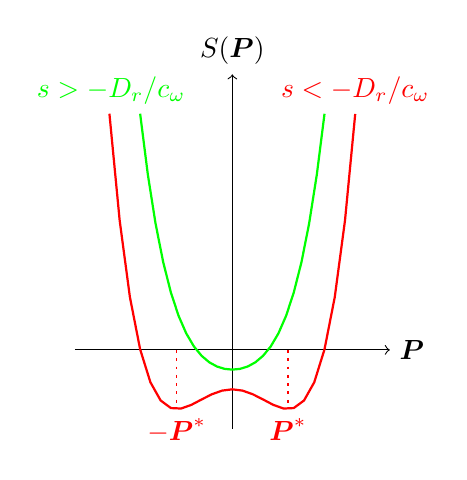
\begin{tikzpicture}

% axes
\draw[->] (0, -1) -- (0, 3.5) node[above]{$S(\boldsymbol{P})$};
\draw[->] (-2, 0) -- (2, 0) node[right]{$\boldsymbol{P}$};

% curves
\draw[thick, green] plot[domain={-sqrt(((sqrt(14) - 1)/2))}:{sqrt(((sqrt(14) - 1)/2))}] (\x, {\x*\x*\x*\x + \x*\x - 0.25});
\draw[green] ({-sqrt(((sqrt(14) + 1)/2))}, 3) node[above]{$s > -D_r/c_{\omega}$};
\draw[thick, red] plot[domain={-sqrt(((sqrt(15) + 1)/2))}:{sqrt(((sqrt(15) + 1)/2))}] (\x, {\x*\x*\x*\x - \x*\x - 0.5});
\draw[red] ({sqrt(((sqrt(15) + 1)/2))}, 3) node[above]{$s < -D_r/c_{\omega}$};

% P^*
\draw[dashed, red, line width=.5pt, dash pattern=on 1pt off 2pt] ({-sqrt(1/2)}, 0) -- ({-sqrt(1/2)}, -0.75) node[below]{$-\boldsymbol{P}^*$};
\draw[dashed, red, line width=.5pt, dash pattern=on 1pt off 2pt] ({sqrt(1/2)}, 0) -- ({sqrt(1/2)}, -0.75) node[below]{$\boldsymbol{P}^*$};

\end{tikzpicture}

\end{document}
